\documentclass[]{article}
\usepackage[T1]{fontenc}
\usepackage{lmodern}
\usepackage{amssymb,amsmath}
\usepackage{ifxetex,ifluatex}
\usepackage{fixltx2e} % provides \textsubscript
% use microtype if available
\IfFileExists{microtype.sty}{\usepackage{microtype}}{}
% use upquote if available, for straight quotes in verbatim environments
\IfFileExists{upquote.sty}{\usepackage{upquote}}{}
\ifnum 0\ifxetex 1\fi\ifluatex 1\fi=0 % if pdftex
  \usepackage[utf8]{inputenc}
\else % if luatex or xelatex
  \usepackage{fontspec}
  \ifxetex
    \usepackage{xltxtra,xunicode}
  \fi
  \defaultfontfeatures{Mapping=tex-text,Scale=MatchLowercase}
  \newcommand{\euro}{€}
\fi
\usepackage[margin=0.8in]{geometry}
\usepackage{longtable}
\usepackage{graphicx}
% We will generate all images so they have a width \maxwidth. This means
% that they will get their normal width if they fit onto the page, but
% are scaled down if they would overflow the margins.
\makeatletter
\def\maxwidth{\ifdim\Gin@nat@width>\linewidth\linewidth
\else\Gin@nat@width\fi}
\makeatother
\let\Oldincludegraphics\includegraphics
\renewcommand{\includegraphics}[1]{\Oldincludegraphics[width=\maxwidth]{#1}}
\ifxetex
  \usepackage[setpagesize=false, % page size defined by xetex
              unicode=false, % unicode breaks when used with xetex
              xetex]{hyperref}
\else
  \usepackage[unicode=true]{hyperref}
\fi
\hypersetup{breaklinks=true,
            bookmarks=true,
            pdfauthor={Sriram V - CS11B058},
            pdftitle={Lab 2: Memory Management},
            colorlinks=true,
            urlcolor=blue,
            linkcolor=magenta,
            pdfborder={0 0 0}}
\urlstyle{same}  % don't use monospace font for urls
\setlength{\parindent}{0pt}
\setlength{\parskip}{6pt plus 2pt minus 1pt}
\setlength{\emergencystretch}{3em}  % prevent overfull lines
\setcounter{secnumdepth}{0}

\title{Lab 2: Memory Management}
\author{Sriram V - CS11B058}
\date{}

\begin{document}
\maketitle

\subsection{Exercise 1}

\begin{itemize}
\itemsep1pt\parskip0pt\parsep0pt
\item
  Implemented the code for \texttt{boot\_alloc()}, \texttt{mem\_init()},
  \texttt{page\_init()}, \texttt{page\_alloc()} and
  \texttt{page\_free()} in \texttt{kern/pmap.c}.
\item
  \texttt{assert()} statements are used wherever necessary to ensure
  that assumptions made for a function are true.
\end{itemize}

\begin{enumerate}
\def\labelenumi{\arabic{enumi}.}
\itemsep1pt\parskip0pt\parsep0pt
\item
  \textbf{\texttt{boot\_alloc()}:}

  \begin{itemize}
  \itemsep1pt\parskip0pt\parsep0pt
  \item
    \texttt{boot\_alloc()} is used for memory allocation only when JOS
    is setting up its virtual memory system. As paging is enabled,
    memory is supposed to be allocated only in terms of pages, using the
    \texttt{page\_alloc()} function.
  \item
    \texttt{boot\_alloc()} initializes \texttt{nextfree} (a pointer to
    the virtual address of the next byte of free memory) the first time
    it is called, by pointing to the first page (of size
    \texttt{PGSIZE}) immediately after the kernel's bss segment (whose
    end is pointed to by \texttt{end}, a magic symbol automatically
    generated by the linker).
  \item
    If \texttt{n\textgreater{}0}, \texttt{boot\_alloc()} allocates n
    bytes of memory (rounded up to the nearest multiple of
    \texttt{PGSIZE}) and returns a pointer to the first byte of this
    chunk of allocated memory.
  \item
    If \texttt{n=0}, it returns a pointer to the address pointed to by
    \texttt{nextfree}.
  \item
    While allocating memory, if the virtual address exceeds
    \texttt{0xf0400000} (The rudimentary mapping done in
    \texttt{kern/entry.S} is from \texttt{{[}0x0, 0x00400000)} to
    \texttt{{[}0xf0000000, 0xf0400000)}), then the kernel panics and
    prints an \texttt{out of memory} message.
  \end{itemize}
\item
  \textbf{\texttt{mem\_init()}:}

  \begin{itemize}
  \itemsep1pt\parskip0pt\parsep0pt
  \item
    The page directory is allocated memory first, using
    \texttt{boot\_alloc()}, and its permissions are set. It is aloso
    recursively inserted in itself as a page table. Its permissions are
    set as well.
  \item
    The first line of code we had to add in was to use
    \texttt{boot\_alloc()} to allocate memory for \texttt{npages} of
    \texttt{PageInfo} structures. This array is pointed to by the
    \texttt{pages} variable.
  \item
    The kernel has a \texttt{PageInfo} structure associated with every
    physical page, to store the page's details such as the physical
    address and the number of references to the page.
  \item
    \texttt{npage} and \texttt{npage\_basemem} are variables that give
    us the ammount of base and physical memory (respectively) in terms
    of number of pages. These values are calculated in
    \texttt{i386\_detect\_memory()}.
  \item
    Then \texttt{page\_init()} is called to initialise \texttt{pages}
    with the data associated with the currently allocated pages.
  \item
    Checks are then performed.
  \end{itemize}
\item
  \textbf{\texttt{page\_init()}:}

  \begin{itemize}
  \itemsep1pt\parskip0pt\parsep0pt
  \item
    The first page is ignored as it is in use. (It contains the
    real-mode IDT and BIOS structures. We preserve them in case we ever
    need them.)
  \item
    The rest of the base memory is then marked as free by adding them to
    \texttt{page\_free\_list}. Page refs are set to zero.
  \item
    We don't allocate pages for the IO hole, which is memory meant for
    IO devices.
  \item
    We query the virtual address of the next byte of free memory (using
    \texttt{boot\_alloc()}), and set all the pages from this one
    onwards, right up to the last page.
  \end{itemize}
\item
  \textbf{\texttt{page\_alloc()}:}

  \begin{itemize}
  \itemsep1pt\parskip0pt\parsep0pt
  \item
    This function first gets the address of the first free page (using
    the pointer to the linked list of free pages -
    \texttt{page\_free\_list}).
  \item
    It shifts this pointer to the next free page as the topmost one has
    now been allocated.
  \item
    If \texttt{alloc\_flags} has a value of \texttt{ALLOC\_ZERO}, then
    the allocated page is filled with \texttt{\textbackslash{}0}s using
    the \texttt{memset()} function.
  \item
    \texttt{memset()} requires the kernel virtual address of the page,
    which is obtained by using the \texttt{page2kva()} function.
  \item
    A \texttt{PageInfo} structure is returned.
  \end{itemize}
\item
  \textbf{\texttt{page\_free()}:}

  \begin{itemize}
  \itemsep1pt\parskip0pt\parsep0pt
  \item
    This function returns a page back to the free list.
  \item
    We first ensure that the \texttt{PageInfo} exists, and that the
    number of references to it are zero, so that we don't accidentally
    free up a page that still has references to it.
  \item
    Once these two points are asserted, we add the page to the list of
    free pages (\texttt{page\_free\_list}).
  \end{itemize}
\end{enumerate}

\subsection{Exercise 2}

\begin{itemize}
\itemsep1pt\parskip0pt\parsep0pt
\item
  \textbf{Page Translation:}

  \begin{itemize}
  \itemsep1pt\parskip0pt\parsep0pt
  \item
    It is in effect only when the \texttt{PG} bit of \texttt{CR0} is
    set.
  \item
    A virtual address is translated into a linear address by the
    segmentation mechanism into a linear address.
  \item
    This linear address maps to a physical address by means of a page
    translation mechanism.
  \item
    The first 10 bits of the 32-bit linear address points gives the
    offset of the entry in the Page Directory. This entry points to a
    Page Table.
  \item
    The next 10 bits of the linear address gives the offset of the Page
    Table Entry, which points to the physical address of the page being
    referred to.
  \item
    The last 12 bits of the linear address gives the offset of the
    physical address within the page.
  \end{itemize}
\item
  \textbf{Page-based Protection:}

  \begin{itemize}
  \itemsep1pt\parskip0pt\parsep0pt
  \item
    Page-level protection is implemented by setting certain bits in the
    32-bit entries in the Page Directory and Page Tables.
  \item
    It is used for both inter and intra-process protection.
  \end{itemize}

  \begin{figure}[htbp]
  \centering
  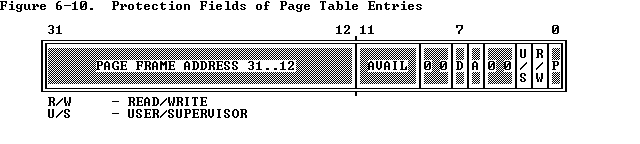
\includegraphics{fig.jpg}
  \caption{Protection Fields of Page Table Entries}
  \end{figure}
\item
  \textbf{Segmentation:}

  \begin{itemize}
  \itemsep1pt\parskip0pt\parsep0pt
  \item
    Segmentation is used for intra-process protection.
  \item
    Different portions of the program are put into different segments.
  \item
    While converting the virtual address to a linear address, the 16
    bits are used to select the segment, and the 32 bits are used to
    offset into the segment.
  \item
    The segment selector points to a segment descriptor that contains
    the base address of the segment, as well as other details such as
    protection and permission bits.
  \end{itemize}
\end{itemize}

\subsection{Exercise 3}

\begin{itemize}
\itemsep1pt\parskip0pt\parsep0pt
\item
  Used \texttt{info pg} in the QEMU monitor (accessed by using
  \texttt{Ctrl-a c}) to view the mapping between the virtual addresses
  and the physical addresses, and the permissions of the pages.
\item
  Used \texttt{xp/i \textless{}physical\_address\textgreater{}} in the
  QEMU monitor, and
  \texttt{x/i \textless{}corresponding\_virtual\_address\textgreater{}}
  in GDB to ensure that both the addresses accessed the same memory
  location.
\end{itemize}

\subsubsection{Questions}

\begin{enumerate}
\def\labelenumi{\arabic{enumi}.}
\item
  \textbf{Assuming that the following JOS kernel code is correct, what
  type should variable \texttt{x} have, \texttt{uintptr\_t} or
  \texttt{physaddr\_t}?}

\begin{verbatim}
    mystery_t x;
    char* value = return_a_pointer();
    *value = 10;
    x = (mystery_t) value;
\end{verbatim}
\end{enumerate}

\begin{itemize}
\itemsep1pt\parskip0pt\parsep0pt
\item
  \texttt{x} should be of the type \texttt{uintptr\_t}, since all
  addresses referred to in C code are virtual addresses and not physical
  addresses.
\end{itemize}

\subsection{Exercise 4}

\begin{itemize}
\itemsep1pt\parskip0pt\parsep0pt
\item
  Implemented code in \texttt{kern/pmap.c} for \texttt{pgdir\_walk()},
  \texttt{boot\_map\_region()}, \texttt{page\_lookup()},
  \texttt{page\_remove()} and \texttt{page\_insert()}.
\end{itemize}

\begin{enumerate}
\def\labelenumi{\arabic{enumi}.}
\itemsep1pt\parskip0pt\parsep0pt
\item
  \textbf{\texttt{pgdir\_walk()}:}

  \begin{itemize}
  \itemsep1pt\parskip0pt\parsep0pt
  \item
    This function returns a pointer to the Page Table Entry, given a
    pointer to a page directory and a linear address.
  \item
    Macros from \texttt{inc/mmu.h} are made use of to manipulate the
    page directory and table entries.
  \item
    \texttt{PDX} is used to get the Page Directory Index for the virtual
    address \texttt{va}.
  \item
    This index is used to then obtain the Page Directory Entry at that
    index.
  \item
    A check is done if a Page Table exists at that entry. If it does, we
    get its kernel virtual address.
  \item
    If it doesn't and the \texttt{create} parameter is \texttt{1}, then
    a new page is allocated using \texttt{page\_alloc()} and filled with
    \texttt{\textbackslash{}0}s.
  \item
    This created page is then inserted into the Page Directory at the
    Page Directory Index with the appropriate permissions, and its
    reference count is incremented by one.
  \item
    In either case, the Page Table Index (obtained by using \texttt{PTX}
    on \texttt{va}) is used to index into the page table, to access the
    corresponding Page Table Entry.
  \item
    A pointer to this entry is returned.
  \item
    In any other case, a \texttt{NULL} is returned.
  \item
    We use \texttt{pte\_t} and \texttt{pde\_t} (\texttt{typedef}s of
    \texttt{uint\_32}) to explicitly specify if we are dealing with a
    page directory or table entry.
  \end{itemize}
\item
  \textbf{\texttt{boot\_map\_region()}:}

  \begin{itemize}
  \itemsep1pt\parskip0pt\parsep0pt
  \item
    This function maps a virtual address range to a physical address
    region with certain permissions for the pages.
  \item
    Assertions are made that the virtual address and physical address
    starts at a multiple of \texttt{PGSIZE}, and that the range is a
    multiple of \texttt{PGSIZE} as well.
  \item
    Starting from the lower value of the virtual address range, we
    identify the corresponding page table entry (using
    \texttt{pgdir\_walk} on the Page Directory, and create a Page Table
    for the entry if one doesn't exist), set the entry to associate with
    the appropriate physical address for that page, set the permissions
    for that entry, and move on to the next page.
  \item
    We do this until the entire virtual address range specified has been
    mapped on to the provided physical address range.
  \end{itemize}
\item
  \textbf{\texttt{page\_lookup()}:}

  \begin{itemize}
  \itemsep1pt\parskip0pt\parsep0pt
  \item
    This function returns the \texttt{PageInfo} structure located at a
    virtual address \texttt{va}, given the Page Directory
    \texttt{pgdir}.
  \item
    \texttt{pgdir\_walk} is used to fetch the pointer to the page table
    entry for the virtual address. Since it is a lookup, the
    \texttt{create} parameter is set to zero.
  \item
    If the page table doesn't exist or a page doesn't exist at the
    corresponding PTE, we return \texttt{NULL}.
  \item
    If it does exist, we find the physical address of the PTE (using the
    macro \texttt{PTE\_ADDR()}) and use the \texttt{pa2page()} function
    to find the corresponding \texttt{PageInfo} structure, which we then
    return as the result.
  \end{itemize}
\item
  \textbf{\texttt{page\_remove()}:}

  \begin{itemize}
  \itemsep1pt\parskip0pt\parsep0pt
  \item
    This function unmaps the page located at the virtual address
    \texttt{va}. If a physical page doesn't exist at this location, it
    fails silently.
  \item
    \texttt{page\_lookup} is used to identify the \texttt{PageInfo}
    structure associated with the page at the virtual address
    \texttt{va}.
  \item
    If a Page Table or Page Table Entry doesn't exist, the funtion
    \texttt{return}s.
  \item
    Else, we decrement the reference count for the structure. This is
    managed using the \texttt{page\_decref()} function, which also frees
    up the page (using \texttt{page\_free()}) if the reference count
    drops to zero.
  \item
    The corresponding Page Table Entry for this page is then set to
    zero, and the TLB is invalidated for the passed virtual address by
    the \texttt{tlb\_invalidate()} function.
  \end{itemize}
\item
  \textbf{\texttt{page\_insert()}:}

  \begin{itemize}
  \itemsep1pt\parskip0pt\parsep0pt
  \item
    This function maps a \texttt{PageInfo} object \texttt{pp} to a
    virtual address \texttt{va}. This is an alternative to the
    \texttt{boot\_map\_region()} function, which maps physical address
    ranges to virtual address ranges. This can be used when the page
    object is known, but its physical address isn't.
  \item
    First we assert that the Page Directory and the \texttt{PageInfo}
    object exist.
  \item
    \texttt{pgdir\_walk()} is then used (with \texttt{create=1}) to find
    the Page Table Entry for the passed virtual address.
  \item
    \texttt{-E\_NO\_MEM} is returned if the Page Table doesn't exist.
    (This can happen only if we run out of memory, as we are explicitly
    requesting the \texttt{pgdir\_walk()} function to create a page
    table if it doesn't exist.)
  \item
    If the Page Table exists and the Page Table Entry exists as well, we
    check if the physical address of the PTE is the same as the physical
    address of the \texttt{PageInfo} object to be inserted.
  \item
    This is a corner case. If we handle it like any other page and
    remove it before adding it back in, we may end up deleting the
    \texttt{PageInfo} object itself.
  \item
    This can happen if the object has its reference count equal to 1. In
    such a case, deleting the PTE using the \texttt{page\_remove()}
    function decrements the reference count for the object to zero,
    which returns the page to the list of free pages, even though it is
    to be reallocated to the same virtual address.
  \item
    Hence, as the object has been marked as a free page, we can no
    longer access the page to increment its reference count and assign
    permissions to it.
  \item
    If it is, it is a case of reinsertion of the same page at the same
    virtual address in the same Page Directory. This means that only a
    permission change for the page is to be effected. Hence, we use a
    \texttt{goto} to jump to the permission change portion.
  \item
    If the physical address of the PTE doesn't match that of the page to
    be inserted, then the page that exists at the virtual address is a
    different page from the one to be inserted. Hence, we call
    \texttt{page\_remove()} to remove the page at this location and to
    invalidate the TLB.
  \item
    We now set the Page Table Entry to point to the physical address of
    the \texttt{PageInfo} object and set the permissions of the PTE. For
    the corner case, this is the only step that happens, i.e., only a
    permission change occurs.
  \item
    A \texttt{0} is returned to signal a successful page insertion.
  \end{itemize}
\end{enumerate}

\subsection{Exercise 5}

\begin{itemize}
\itemsep1pt\parskip0pt\parsep0pt
\item
  Now that all the helper functions have been filled in, we can duly
  fill in the rest of the \texttt{mem\_init()} function after the call
  to \texttt{check\_page()}.
\item
  The code we write now initializes the kernel address space.
\item
  The kernel virtual address space is mapped to corresponding physical
  address regions by making use of the \texttt{map\_boot\_region()}
  function.
\item
  The \texttt{pages} array that contains all the \texttt{PageInfo}
  objects is mapped to the virtual address given by the macro
  \texttt{UPAGES}.
\item
  This region is provided as Read Only for both the kernel and the user,
  as it is a means for the user to access the kernel data structures.
\item
  The actual physical address that this virtual address maps to has RW
  permissions for the kernel, so that the kernel can modify the data
  structures here. This region is inaccessible by the user.
\item
  The changes made here are reflected at the mapped virtual address,
  which can be read by the user. Hence, a protected interface for kernel
  methods is provided to the user.
\item
  The next mapping maps the kernel stack (physical address is given by
  the \texttt{bootstack} variable set in \texttt{kern/entry.S}) to the
  virtual address \texttt{KSTACKTOP}. The region mapped is of size
  \texttt{KSTKSIZE}, rather than \texttt{PTSIZE}.
\item
  This is because the region
  \texttt{{[}KSTACKTOP-PTSIZE, KSTACKTOP-KSTKSIZE)} is meant to be a
  `guard page' - this page doesn't have a corresponding physical page
  (not backed by the physical memory), so if the kernel overflows its
  stack, a fault will occur rather than overwriting of memory (since
  virtual memory to write into exists, but corresponding physical memory
  doesn't).
\item
  Since it is the kernel stack, the kernel has RW permissions, but the
  user has none.
\item
  The final mapping is to map the virtual address range
  \texttt{{[}KERNBASE, 2\^{}32)} to the physical address range
  \texttt{{[}0, 2\^{}32 - KERNBASE)}. This is done to replace the
  rudimentary mapping that was done in \texttt{kern/entry.S}, before the
  page directory and tables were allocated and initialised.
\item
  Also, when we switch from the rudimentary mapping to the full-fledged
  page directory that has just been created, we will not have any
  issues, as the virtual addresses pointed to by the old page directory
  (in range \texttt{{[}0xf0000000, 0xf0400000)}) will still map to the
  same physical address range \texttt{{[}0x00000000, 0x00400000)} as
  before.
\end{itemize}

\subsubsection{Questions}

\begin{enumerate}
\def\labelenumi{\arabic{enumi}.}
\setcounter{enumi}{1}
\itemsep1pt\parskip0pt\parsep0pt
\item
  \textbf{What entries (rows) in the page directory have been filled in
  at this point? What addresses do they map and where do they point? In
  other words, fill out the table as much as possible:}
\end{enumerate}

\begin{itemize}
\item
  Filled table:

  \begin{longtable}[c]{@{}ccc@{}}
  \hline\noalign{\medskip}
  Entry & Base Virtual Address & Points to (logically)
  \\\noalign{\medskip}
  \hline\noalign{\medskip}
  1023 & \texttt{0xffc00000} & Page table for top 4MB of phys memory
  \\\noalign{\medskip}
  . & \texttt{.} & \texttt{.}
  \\\noalign{\medskip}
  . & \texttt{.} & \texttt{.}
  \\\noalign{\medskip}
  . & \texttt{.} & \texttt{.}
  \\\noalign{\medskip}
  960 & \texttt{0xf0000000} & \texttt{KERNBASE}
  \\\noalign{\medskip}
  959 & \texttt{0xefc00000} & \texttt{VPT,KSTACKTOP}
  \\\noalign{\medskip}
  958 & \texttt{0xef800000} & \texttt{ULIM}
  \\\noalign{\medskip}
  957 & \texttt{0xef400000} & \texttt{UVPT}
  \\\noalign{\medskip}
  956 & \texttt{0xef000000} & \texttt{UPAGES (RO PAGES)}
  \\\noalign{\medskip}
  955 & \texttt{0xeec00000} & \texttt{UTOP,UENVS/UXSTACKTOP (RO ENVS)}
  \\\noalign{\medskip}
  . & \texttt{.} & \texttt{.}
  \\\noalign{\medskip}
  . & \texttt{.} & \texttt{.}
  \\\noalign{\medskip}
  . & \texttt{.} & \texttt{.}
  \\\noalign{\medskip}
  2 & \texttt{0x00800000} & \texttt{UTEXT}
  \\\noalign{\medskip}
  1 & \texttt{0x00400000} & \texttt{UTEMP}
  \\\noalign{\medskip}
  0 & \texttt{0x00000000} & Real-mode \texttt{IDT}, \texttt{BIOS} etc.
  \\\noalign{\medskip}
  \hline
  \end{longtable}
\end{itemize}

\begin{enumerate}
\def\labelenumi{\arabic{enumi}.}
\setcounter{enumi}{2}
\itemsep1pt\parskip0pt\parsep0pt
\item
  \textbf{We have placed the kernel and user environment in the same
  address space. Why will user programs not be able to read or write the
  kernel's memory? What specific mechanisms protect the kernel memory?}
\end{enumerate}

\begin{itemize}
\itemsep1pt\parskip0pt\parsep0pt
\item
  The virtual memory is divided into segments by ULIM and UTOP -
  \texttt{(ULIM, 4GB)} is Kernel only, \texttt{(UTOP, ULIM{]}} can be
  accessed by both the Kernel and User environment (Read Only) and
  \texttt{{[}0x0, UTOP{]}} is user environment space.
\item
  These memory spaces are protected by the permission bits, such as
  \texttt{PTE\_W} (writeable) and \texttt{PTE\_U} (user), which are set
  in the page table/directory entries.
\item
  The Current Privilege Level (CPL) is used to identify whether in
  privileged mode (\texttt{CPL=0} - the kernel) or not (\texttt{CPL=3} -
  user processes). Accordingly, certain pages in the memory are (or are
  not) accessible.
\end{itemize}

\begin{enumerate}
\def\labelenumi{\arabic{enumi}.}
\setcounter{enumi}{3}
\itemsep1pt\parskip0pt\parsep0pt
\item
  \textbf{What is the maximum amount of physical memory that this
  operating system can support? Why?}
\end{enumerate}

\begin{itemize}
\itemsep1pt\parskip0pt\parsep0pt
\item
  Since \texttt{KERNBASE} is equal to \texttt{0xf0000000}, the virtual
  address range mentioned above has a size of approximately 256MB.
  Hence, the physical range it maps to has to have a size of 256MB as
  well.
\item
  If we have physical memory greater than 256MB, then there will be a
  region that is unmapped.
\item
  Reverse mappings from certain physical addresses to virtual addresses
  would not exist. The unmapped region would not be usable.
\item
  Thus, this operating system can support only upto 256MB.
\end{itemize}

\begin{enumerate}
\def\labelenumi{\arabic{enumi}.}
\setcounter{enumi}{4}
\itemsep1pt\parskip0pt\parsep0pt
\item
  \textbf{How much space overhead is there for managing memory, if we
  actually had the maximum amount of physical memory? How is this
  overhead broken down?}
\end{enumerate}

\begin{itemize}
\itemsep1pt\parskip0pt\parsep0pt
\item
  Memory management is handled by means of the Page Directory and the
  associated page tables.
\item
  We have a single page directory, and this accounts for 4KB.
\item
  Since the page directory can have a maximum of 1024 entries, if we had
  the maximum amount of physical memory, all these entries would be
  filled up.
\item
  Hence, we would also be having 1024 page tables, each of size 4KB.
  Therefore the total space overhead is \texttt{4KB * 1024 + 4KB}, which
  is 4KB more than 4MB i.e., the space overhead would be a little over
  4MB.
\end{itemize}

\begin{enumerate}
\def\labelenumi{\arabic{enumi}.}
\setcounter{enumi}{5}
\itemsep1pt\parskip0pt\parsep0pt
\item
  \textbf{Revisit the page table setup in \texttt{kern/entry.S} and
  \texttt{kern/entrypgdir.c}. Immediately after we turn on paging,
  \texttt{EIP} is still a low number (a little over 1MB). At what point
  do we transition to running at an \texttt{EIP} above
  \texttt{KERNBASE}? What makes it possible for us to continue executing
  at a low \texttt{EIP} between when we enable paging and when we begin
  running at an \texttt{EIP} above \texttt{KERNBASE}? Why is this
  transition necessary?}
\end{enumerate}

\begin{itemize}
\itemsep1pt\parskip0pt\parsep0pt
\item
  We transition to running at an EIP above KERNBASE once paging is
  enabled and just before entering the C code (\texttt{line 68} in
  \texttt{kern/entry.S}).
\item
  A trivial page directory (defined in \texttt{/kern/entrypgdir.c}) is
  loaded into CR3 before paging is enabled. This code defines the
  initial PD and PT that are used in \texttt{kern/entry.S}
\item
  This code maps both \texttt{{[}0, 4MB)} and
  \texttt{{[}KERNBASE, KERNBASE+4MB)} sets of VAs to the
  \texttt{{[}0, 4MB)} set of PAs.
\item
  So after paging is enabled, the low virtual addresses are still being
  mapped to the correct low physical addresses.
\item
  Hence, execution at a low \texttt{EIP} after enabling paging makes it
  possible to continue execution.
\item
  This transition is necessary so that the kernel can be run at a high
  virtual address. It must run at a high virtual address because the
  lower address space is meant for user code in the x86 atchitecture, so
  by accessing it from a large virtual address, the lower addresses are
  free for user processes.
\end{itemize}

\end{document}
